%%%%%%%%%%%%%%
% LECTURE 11 %
%%%%%%%%%%%%%%
\vspace{1cm}
\noindent\lecture{11}{12/11/2021}

\subsection{Amplitude damping}
Un'importante applicazione delle \textbf{quantum operations} è la descrizione della dissipazione di energia, ossia effetti dovuti alla perdita di energia da un sistema quantistico. Quali sono le dinamiche di un atomo che emette spontaneamente un fotone? In che modo un sistema di spin ad alta temperatura si avvicina all'equilibrio con il suo ambiente? Qual è lo stato di un fotone in un interferometro o in una cavità quando è soggetto a diffusione e attenuazione? Ciascuno di questi processi ha le sue caratteristiche uniche, ma il comportamento generale di un qubit è ben caratterizzato da un'operazione quantistica nota come \textbf{amplitude damping} (smorzamento dell'ampiezza), che possiamo ricavare considerando il caso dell'emissione spontanea nella seguente schematizzazione:
\begin{center}
    $
        \begin{matrix}
             \\
             \\
            \begin{Large}\substack{\text{Emissione} \\ \text{spontanea}}\end{Large}: \\
        \end{matrix}
        $
    \raisebox{1.2em}{
        \mbox{
            \Qcircuit @C=2em @R=2em {
                & \qw & \rstick{\ket{1}} \qw \\
                & \raisebox{.3em}{\begin{huge}$\downarrow$\end{huge}} & \raisebox{.05em}{\begin{huge} $\rightsquigarrow$ \end{huge}}\\
                & \qw & \rstick{\ket{0}} \qw
            }
        }
    }
\end{center}
\vspace{0.2cm}
dove, d'ora in avanti, assumeremo che lo stato $\ket{1}$ ha un'energia associata maggiore di quella dello stato $\ket{0}$. Possiamo descrivere la fisica dell’emissione spontanea dal punto di vista dell’ambiente nel modo seguente: assumiamo che esso presenti una base ortonormale costituita dai due stati seguenti
\begin{align*}
    \ket{0}_E &= \text{Nessuna emissione di fotoni}. \\
    \ket{1}_E &= \text{1 fotone emesso}. 
\end{align*}
In questo modo il sistema totale $\mathcal{H}_q \otimes \mathcal{H}_E$ evolve con un'evoluzione unitaria $U$ tale che
\begin{equation}\label{variazione_stati_emissione_spontanea}
    U \, : \; 
    \begin{cases}
        \ket{0} \otimes \ket{0}_E &\rightarrow  \ket{0} \otimes \ket{0}_E \\
        \ket{1} \otimes \ket{0}_E &\rightarrow  \sqrt{1-p} \ket{1} \otimes \ket{0}_E + \sqrt{p} \ket{0} \otimes \ket{1}_E
    \end{cases} \, ;
\end{equation}
nel primo caso non succede nulla, il nostro sistema è nello stato fondamentale per cui non ci sarà mai emissione di fotoni. Nel secondo caso, invece, c'è una probabilità $p$ che il nostro sistema, essendo nello stato eccitato, emetta spontaneamente un fotone, per cui dopo si troverà nello stato fondamentale, e una probabilità $1-p$ che il nostro sistema rimanga nello stato eccitato senza alcuna emissione di fotoni. Precisiamo che le trasformazioni \eqref{variazione_stati_emissione_spontanea} sono unitarie: è immediatamente evidente che, essendo ciascun stato ortogonale agli altri, il prodotto scalare è conservato. Come al solito, siamo interessati a studiare il nostro sistema ignorando i gradi di libertà dell'ambiente, per cui valutiamo la traccia parziale su $\mathcal{H}_E$ mediante il calcolo degli operation elements \eqref{E_k}. Per semplicità di scrittura identifichiamo $\ket{e_0} \equiv \ket{0}_E$ e $\ket{e_1} \equiv \ket{1}_E$. Prima di procedere ricordiamo che $E_k=\mel{e_k}{U}{e_0}$ è equivalente a scrivere $\mel{x}{E_k}{y}=\mel{xe_k}{U}{ye_0}$, dove $\ket x , \ket y \in \mathcal{H}_q$, dunque abbiamo un modo operativo per poter calcolare ciascun termine. Valutiamo le matrici $E_0$ ed $E_1$:
\begin{align*}
    E_0 &= {}_E \! \mel{0}{U}{0}_E &\Rightarrow& \;
    \begin{cases}
        \mel{0}{E_0}{0}=\mel{00}{U}{00}=1 \\
        \mel{1}{E_0}{1}=\mel{10}{U}{10}=\sqrt{1-p} \\
        \mel{0}{E_0}{1}=\mel{00}{U}{10}=0 \\
        \mel{1}{E_0}{0}=\mel{10}{U}{00}=0
    \end{cases}
    &\Rightarrow&
    &E_0 &= 
    \begin{pmatrix}
        1 & 0 \\
        0 & \sqrt{1-p}
    \end{pmatrix} , \\
    E_1 &= {}_E \! \mel{1}{U}{0}_E &\Rightarrow& \;
    \begin{cases}
        \mel{0}{E_1}{0}=\mel{01}{U}{00}=0 \\
        \mel{1}{E_1}{1}=\mel{11}{U}{10}=0 \\
        \mel{0}{E_1}{1}=\mel{01}{U}{10}=\sqrt p \\
        \mel{1}{E_1}{0}=\mel{11}{U}{00}=0
    \end{cases}
    &\Rightarrow& 
    &E_1 &= 
    \begin{pmatrix}
        0 & \sqrt p \\
        0 & 0
    \end{pmatrix} \, .
\end{align*}
Per verificare se quanto ottenuto sia consistente possiamo controllare che le matrici soddisfino il vincolo \eqref{constraint_E_k}
\begin{equation*}
    \sum_k E_k^\dagger E_k = E_0^\dagger E_0+E_1^\dagger E_1 = 
    \begin{pmatrix}
    1 & 0 \\
    0 & 1-p
    \end{pmatrix} +
    \begin{pmatrix}
    0 & 0 \\
    0 & p
    \end{pmatrix}
    = \mathbb{I} \, .
\end{equation*}
A questo punto siamo pronti a valutare $\mathcal{E}(\rho)$ per mezzo della \eqref{operator_sum_repr}. Consideriamo una generica matrice densità
\begin{equation*}
    \rho = \begin{pmatrix}
    \rho_{00} & \rho_{01} \\
    \rho_{10} & \rho_{11}
    \end{pmatrix} \, ,
\end{equation*}
e andiamo a calcolare la sua trasformazione:
\begin{align}
    \mathcal{E}(\rho) &= \sum_k E_k \rho E_k^\dagger = E_0\rho E_0^\dagger + E_1\rho E_1^\dagger \notag \\
    &= \begin{pmatrix}
            \rho_{00} & \sqrt{1-p} \rho_{01} \\
            \sqrt{1-p}\rho_{10} & (1-p)\rho_{11}
        \end{pmatrix}
        +
        \begin{pmatrix}
            p\rho_{11} & 0 \\
            0 & 0
        \end{pmatrix} \notag \\
    &= \begin{pmatrix}
            \rho_{00}+p\rho_{11} & \sqrt{1-p}\rho_{01} \\
            \sqrt{1-p}\rho_{10} & (1-p)\rho_{11}
        \end{pmatrix}  \, . \label{rho-damping}
\end{align}
Scritta in questo modo, $\mathcal{E}(\rho)$ risulta di difficile interpretazione fisica, quindi solitamente quello che si fa in QM è introdurre una \textit{probabilità di decadimento per unità di tempo}, detta $\Gamma$, tale per cui la probabilità $p$ che avvenga un'emissione spontanea risulti definita come $p=\Gamma \Delta t$. Ma $\Gamma$ definita così lo è per tempi infinitesimi, quindi per poterla usare per tempi finiti dobbiamo valutarla su un lasso di tempo finito $t = n \Delta t$, dove $n$ è il numero di intervalli considerati, e mandare $n \to \infty$. A questo punto, ricordando che in ogni intervallo abbiamo una probabilità di $1-p$ che il decadimento non avvenga, in un tempo finito avremo
\begin{equation*}
    (1-p)^n = \left(1- \Gamma \Delta t \right)^n = \left(1-\frac{\Gamma t}{n}\right)^n \overset{n \to \infty}{\longrightarrow} e^{-\Gamma t} \, ,
\end{equation*}
quindi $(1-p) = e^{-\Gamma t}$. Con questa nuova definizione possiamo riscrivere la \eqref{rho-damping} come
\begin{equation}\label{rho-damping2}
    \mathcal{E}(\rho) = \begin{pmatrix}
                            \rho_{00}+(1-e^{-\Gamma t})\rho_{11} & e^{-\frac{\Gamma t}{2}}\rho_{01} \\
                            e^{-\frac{\Gamma t}{2}}\rho_{10} & e^{-\Gamma t}\rho_{11}
                        \end{pmatrix} \, ;
\end{equation}
osserviamo che gli elementi sulla diagonale contengono $\Gamma$ mentre quelli off-diagonal $\Gamma/2$. Possiamo definire anche il \textit{tempo di vita} come $\Gamma = 1/T$ dimodoché $e^{-\Gamma t}=e^{-t/T}$. Vediamo cosa succede per tempi molto grandi:
\begin{equation*}
    \mathcal{E}(\rho) \overset{t \to \infty}{\longrightarrow} 
    \begin{pmatrix}
        \rho_{00}+\rho_{11} & 0 \\
        0 & 0
    \end{pmatrix} =
    \begin{pmatrix}
        1 & 0 \\
        0 & 0
    \end{pmatrix}
    = \op{0}{0} \, ,
\end{equation*}
dove nel secondo passaggio abbiamo fatto uso di $\Tr \rho = 1$ (si ricordi anche che essendo $\mathcal{E}(\rho)$ una matrice densità deve valere $\Tr \mathcal{E}(\rho) = 1$). 
Il motivo per cui abbiamo ottenuto una matrice densità corrispondente ad uno stato puro è molto semplice: se lasciamo che il qubit interagisca con l'ambiente per un lungo periodo di tempo, allora, con probabilità 1, se si trova nello stato eccitato decadrà sempre nel suo stato fondamentale emettendo un fotone. In termini della sfera di Bloch, il processo è rappresentato in Figura \ref{fig:shrinking_to_0}.

\begin{figure}[!h]
    \centering
    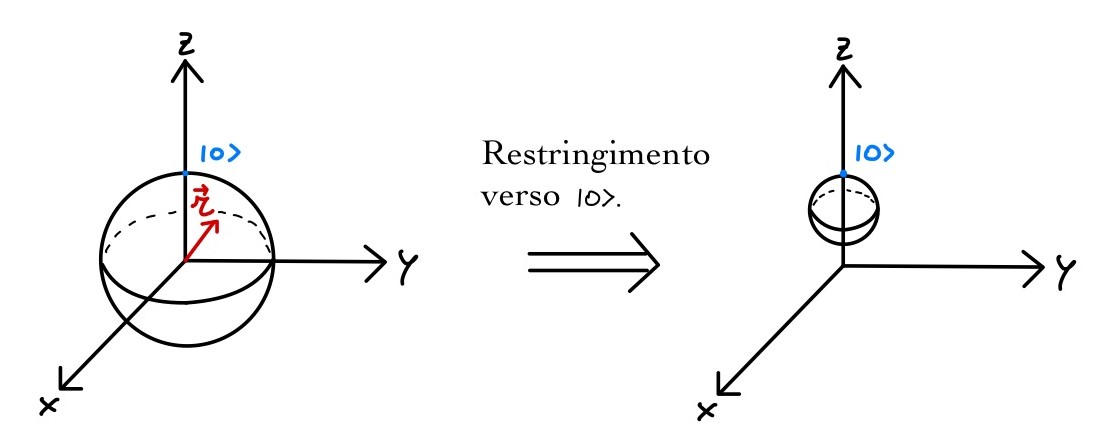
\includegraphics[scale=0.4]{images/shrinking_to_0}
    \caption{La sfera di Bloch si restringe verso lo stato $\ket{0}$ per tempi molto lunghi.}
    \label{fig:shrinking_to_0}
\end{figure}


\subsection{Phase damping}
Un processo di rumore che è unicamente quantistico e descrive la perdita di \textit{coerenza}, ossia di informazioni quantistiche senza perdita di energia, è il \textbf{phase damping} (smorzamento della fase). Fisicamente descrive, ad esempio, cosa succede quando un fotone si disperde casualmente mentre viaggia attraverso una guida d'onda, o come gli stati elettronici in un atomo vengono perturbati quando interagisce con cariche elettriche distanti. Gli autostati energetici di un sistema quantistico non cambiano in funzione del tempo, ma accumulano una fase proporzionale all'autovalore. Quando un sistema evolve per un periodo di tempo non noto con precisione, le informazioni parziali su questa fase relativa, tra gli autostati energetici, vengono perse, quindi questo fenomeno affligge unicamente la fase relativa di una sovrapposizione quantistica di stati. 

\noindent In maniera analoga a quanto visto nell'amplitude damping, possiamo descrivere la fisica dietro al phase damping considerando lo scattering di particelle presenti nell'ambiente con il nostro sistema quantistico. Modelliziamo la situazione dal punto di vista dell'ambiente introducendo la seguente base
\begin{align*}
    \ket{0}_E &= \text{Ground state: nessuno scattering}. \\
    \ket{1}_E &= \text{Scattering che porta al I stato eccitato}. \\
    \ket{2}_E &= \text{Scattering che porta al II stato eccitato},
\end{align*}
dove lo stato eccitato finale dell'ambiente dipender\`a dallo stato del qubit.
In questo modo il sistema totale $\mathcal{H}_q \otimes \mathcal{H}_E$ evolve con l'evoluzione unitaria $U$ tale che
\begin{equation}\label{phase_damping}
    U \, : \; 
    \begin{cases}
        \ket{0} \otimes \ket{0}_E &\rightarrow  \sqrt{1-p} \ket{0} \otimes \ket{0}_E + \sqrt{p} \ket{0} \otimes \ket{1}_E \\
        \ket{1} \otimes \ket{0}_E &\rightarrow  \sqrt{1-p} \ket{1} \otimes \ket{0}_E + \sqrt{p} \ket{1} \otimes \ket{2}_E
    \end{cases} \, ;
\end{equation}
abbiamo indicato con $p$ la probabilità che lo scattering cambi in qualche modo lo stato dell'ambiente: in tutti i casi, trattandosi di scattering, il qubit rimane nel suo stato mentre lo stato che descrive l'ambiente cambia. Come nel caso dell'amplitude damping, l'operatore che descrive le trasformazioni \eqref{phase_damping} è unitario poiché i prodotti scalari sono conservati. L'obiettivo è quello di valutare il nostro sistema (qubit) ignorando l'ambiente e lo facciamo prendendo una traccia della matrice densità $\rho$, ancora una volta, su $\mathcal{H}_E$. Calcoliamo gli operation elements della \eqref{E_k} ricordando, come in precedenza, che $E_k = {}_E \! \mel{k}{U}{0}_E \Leftrightarrow \mel{x}{E_k}{y} = \mel{x k}{U}{y 0}$. In questo caso avremo 3 matrici $E_0$, $E_1$ ed $E_2$:
\begin{align*}
    E_0 &= {}_E \! \mel{0}{U}{0}_E &\Rightarrow& \;
    \begin{cases}
        \mel{0}{E_0}{0}=\mel{00}{U}{00}=\sqrt{1-p} \\
        \mel{1}{E_0}{1}=\mel{10}{U}{10}=\sqrt{1-p} \\
        \mel{0}{E_0}{1}=\mel{00}{U}{10}=0 \\
        \mel{1}{E_0}{0}=\mel{10}{U}{00}=0
    \end{cases} 
    &\Rightarrow&
    &E_0 &= \sqrt{1-p}
          \begin{pmatrix}
            1 & 0 \\
            0 & 1
          \end{pmatrix} \, , \\
    E_1 &= {}_E \! \mel{1}{U}{0}_E &\Rightarrow& \;    \begin{cases}
        \mel{0}{E_0}{0}=\mel{01}{U}{00}=\sqrt{p} \\
        \mel{1}{E_0}{1}=\mel{11}{U}{10}=0 \\
        \mel{0}{E_0}{1}=\mel{01}{U}{10}=0 \\
        \mel{1}{E_0}{0}=\mel{11}{U}{00}=0
    \end{cases}
    &\Rightarrow&
    &E_1 &= \sqrt{p}
          \begin{pmatrix}
            1 & 0 \\
            0 & 0
          \end{pmatrix} \, , \\
    E_2 &= {}_E \! \mel{2}{U}{0}_E &\Rightarrow& \;
    \begin{cases}
        \mel{0}{E_0}{0}=\mel{02}{U}{00}=0 \\
        \mel{1}{E_0}{1}=\mel{12}{U}{10}=\sqrt{p} \\
        \mel{0}{E_0}{1}=\mel{02}{U}{10}=0 \\
        \mel{1}{E_0}{0}=\mel{12}{U}{00}=0
    \end{cases}
    &\Rightarrow&
    &E_2 &= \sqrt{p}
          \begin{pmatrix}
            0 & 0 \\
            0 & 1
          \end{pmatrix} \, .
\end{align*}
Le matrici ottenute soddisfano coerentemente la \eqref{constraint_E_k}:
\begin{align*}
    \sum_k E_k^\dagger E_k &= E_0^\dagger E_0 + E_1^\dagger E_1 +  E_2^\dagger E_2 \\
    &=
    \begin{pmatrix}
        1-p & 0 \\
        0 & 1-p
    \end{pmatrix}
    +
    \begin{pmatrix}
        p & 0 \\
        0 & 0
    \end{pmatrix}
    +
    \begin{pmatrix}
        0 & 0 \\
        0 & p
    \end{pmatrix} = \mathbb{I} \, .
\end{align*}
Avendo ora a disposizione $E_0$, $E_1$ ed $E_2$, possiamo calcolare la \eqref{operator_sum_repr}: 
\begin{align}
    \rho \to \mathcal{E}(\rho) &= \sum_k E_k \rho E_k^\dagger = E_0\rho E_0^\dagger + E_1\rho E_1^\dagger + E_2\rho E_2^\dagger \notag \\
    &= (1-p)\rho + p\frac{\mathbb{I}+\sigma_3}{2}\rho\frac{\mathbb{I}+\sigma_3}{2}+p\frac{\mathbb{I}-\sigma_3}{2}\rho\frac{\mathbb{I}-\sigma_3}{2} \notag \\
    &= (1-p)\rho +\frac 12(p\rho + p\sigma_3\rho \sigma_3) \notag \\
    &= \left( 1-\frac p2 \right) \rho +\frac p2 \sigma_3\rho\sigma_3 \, , \label{matrix_rho_p_damping}
\end{align}
dove nella seconda linea abbiamo utilizzato $E_1 =\sqrt{p} \frac{\mathbb{I}+\sigma_3}{2}$ e $E_2 =\sqrt{p} \frac{\mathbb{I}-\sigma_3}{2}$. Questo risultato non è nient'altro che il conto che avevamo svolto nell'Esempio \ref{es:phase_flip} del phase flip channel. Un altro modo per rendere più esplicito questo fatto è quello di introdurre il cambio di variabili $\tilde{p}=1-\frac p2$ nella precedente
\begin{equation}\label{rho-p-damping}
    \mathcal{E}(\rho) = \tilde{p}\rho+(1-\tilde{p})Z\rho Z \, ,
\end{equation}
e ricordare che \texttt{Z-gate} introduce, in un generico stato, una fase relativa
\begin{equation*}
    \alpha\ket 0+ \beta \ket 1 \overset{Z}{\longrightarrow} \alpha \ket 0 - \beta \ket 1 \, ;
\end{equation*}
(si veda direttamente l'Esempio \ref{es:phase_flip} per capire la trasformazione di $\vec{r}$ e visualizzarne l'effetto sulla sfera di Bloch). Perciò, esplicitando la \eqref{matrix_rho_p_damping}, la generica matrice densità si trasformerà nel seguente modo
\begin{equation*}
    \rho = \begin{pmatrix}
                \rho_{00} & \rho_{01} \\
                \rho_{10} & \rho_{11}
           \end{pmatrix}
    \longrightarrow
    \mathcal{E}(\rho) = \begin{pmatrix}
                            \rho_{00} & (1-p)\rho_{01} \\
                            (1-p)\rho_{10} & \rho_{11}
                        \end{pmatrix} \, ;
\end{equation*}
Ancora una volta, possiamo introdurre un'opportuna ampiezza di scattering $\Gamma$ e sostituire la probabilità con il termine di decadimento esponenziale $(1-p)=e^{-\Gamma t}$ nel limite in cui $n \to \infty$:
\begin{equation}\label{rho_final_phase_damping}
    \mathcal{E}(\rho) = \begin{pmatrix}
                            \rho_{00} & e^{-\Gamma t}\rho_{01} \\
                            e^{-\Gamma t}\rho_{10} & \rho_{11}
                        \end{pmatrix} \, ;
\end{equation}
solamente le componenti off-diagonal risentono dell'interazione con l'ambiente a differenza di quanto avveniva nell'amplitude damping! Ricapitolando: una singola azione del phase flip channel produce una singola aggiunta di una fase, tuttavia molte azioni ripetute dell'ambiente (scattering con le particelle) causano una diminuzione delle componenti off-diagonal di $\rho$, ossia una perdita di coerenza nei termini di interferenza degli stati quantistici.

\noindent Evidenziamo un aspetto particolare che è opportuno menzionare e che incontreremo nuovamente nella sezione successiva sulla \textbf{quantum error-correction}. In questa situazione abbiamo ricavato il risultato \eqref{rho-p-damping} da una prospettiva differente rispetto all'Esempio \ref{es:phase_flip} poiché abbiamo visto che lo stato del qubit può essere invertito a seguito degli scattering con le particelle esterne dell'ambiente. Vi è una sorta di \textbf{universalità}: quando, in fisica, si ritrova un comportamento universale è sempre un fatto positivo, tuttavia è bene ricordare che i qubit, a differenza del CC, sono continui (sovrapposizione di stati, gate unitari dipendenti da parametri continui, ecc.) e quindi sembrerebbe molto difficoltoso controllare tutte le possibili situazioni perché si potrebbe ingenuamente pensare che ci siano un'infinità di errori agenti sui qubit! Il punto fondamentale è che se si aspetta un tempo sufficientemente lungo tutti questi effetti sono indistinguibili e si finisce sempre in una delle due situazioni appena esaminate: si perde energia (amplitude damping) o si perde coerenza (phase damping).

\noindent Storicamente, il phase damping era un processo che è stato quasi sempre pensato, fisicamente, come risultato di un processo casuale di kick di fase o scattering. Non lo è stato fino a quando fu scoperta la connessione al phase flip channel, il quale è stato analizzato nella teoria della correzione degli errori quantistici: si pensava infatti che gli errori di fase fossero continui e non potessero quindi essere descritti come un processo discreto! In effetti, gli errori di fase del singolo qubit possono sempre essere pensati come il risultato di un processo in cui, con probabilità $p$, non accade nulla a un qubit o, con probabilità $1-p$, il qubit viene capovolto dallo \texttt{Z-gate}. Sebbene questo potrebbe non essere l'effettivo processo fisico microscopico che sta accadendo, dal punto di vista della trasformazione che si verifica in un qubit su un intervallo di tempo discreto, ampio rispetto al processo casuale sottostante, non c'è alcuna differenza.

\noindent Vediamo un altro esempio di modello molto semplice che produce il medesimo effetto sul qubit, ossia il phase damping e la conseguente perdita di coerenza. Supponiamo di avere un qubit nello stato $\ket \psi = a \ket 0 + b \ket 1$ che interagisce con l'ambiente, il quale aggiunge al qubit delle fasi casuali in qualche direzione particolare, diciamo una rotazione $R_z(\theta) = e^{-\frac{i \theta \sigma_3}{2}}$ attorno a $z$, dove l'angolo di rotazione $\theta$ è casuale:
\begin{equation}\label{rotation_on_coeffs}
    \ket{\psi} \rightarrow R_z(\theta)\ket \psi = e^{-i\frac \theta 2 \sigma_3}\ket \psi = a e^{-i\frac \theta 2} \ket 0 + b e^{i\frac \theta 2} \ket 1 \, ,
\end{equation}
quindi il suo effetto è quello di frapporre una fase relativa tra $\ket{0}$ e $\ket{1}$. Non vogliamo studiare il caso di un valore particolare di $\theta$, ma vogliamo invece capire che cosa succede quando si hanno errori multipli. Consideriamo un'interazione continua con l'ambiente, il quale causa $\ket{\psi} \to R_z(\theta) \ket{\psi}$ per qualche valore casuale di $\theta$, e supponiamo che l'angolo di rotazione sia una variabile casuale con una ben definita distribuzione di probabilità. Immaginiamo che tale distribuzione sia una gaussiana con media $\theta$ e varianza $2\lambda$: la probabilità di avere un angolo $\theta$ è data da
\begin{equation*}
    P(\theta) = \frac{1}{\sqrt{4 \pi \lambda}} e^{-\frac{\theta^2}{4\lambda}} \, .
\end{equation*}
Vediamo cosa succede al qubit aspettando del tempo: l'effetto di una singola rotazione sullo stato finale del qubit dopo questo processo è descritto dalla seguente matrice densità
\begin{equation*}
    \rho = \op{\psi}{\psi} \rightarrow \mathcal{E}(\rho) =  R_z(\theta)\op{\psi}{\psi}R_z^\dagger(\theta) \, ,
\end{equation*}
quindi se integriamo su tutti i valori di $\theta$ possiamo calcolare un effetto totale mediato
\begin{align*}
    \expval{\mathcal{E}(\rho)}_\theta &= \frac{1}{\sqrt{4\pi\lambda}} \int \dd{\theta} e^{-\frac{\theta^2}{4\lambda}}R_z(\theta)\op{\psi}{\psi}R_z^\dagger(\theta) \\
    &= \frac{1}{\sqrt{4\pi\lambda}} \int \dd{\theta} e^{-\frac{\theta^2}{4\lambda}}R_z(\theta)
    \begin{pmatrix}
        \abs{a}^2 & ab^* \\
        a^*b & \abs{b}^2
    \end{pmatrix}
    R_z^\dagger(\theta) \\
    &= \frac{1}{\sqrt{4\pi\lambda}} \int \dd{\theta} e^{-\frac{\theta^2}{4\lambda}}
    \begin{pmatrix}
        \abs{a}^2 & ab^*e^{-i\theta} \\
        a^*be^{i\theta} & \abs{b}^2
    \end{pmatrix} \, ,
\end{align*}
dove nell'ultima riga abbiamo letto l'effetto di $R_z(\theta)$ su $a$ e $b$ dalla \eqref{rotation_on_coeffs}: $a \to a e^{-i\theta/2}$ e $b \to b e^{i \theta/2}$. L'integrale dei termini diagonali è banale perché cancella esattamente la normalizzazione, mentre l'integrale dei termini off-diagonal è un semplice integrale gaussiano
\begin{equation*}
    \frac{1}{\sqrt{4\pi\lambda}} \int \dd{\theta} e^{-\frac{\theta^2}{4\lambda} \pm i \theta} = \frac{1}{\sqrt{4\pi\lambda}} \int \dd{\theta} e^{-\frac{1}{4\lambda}(\theta \mp 2 \lambda i)^2 - \lambda} = e^{-\lambda} \, ,
\end{equation*}
dove nel penultimo passaggio abbiamo ricostruito il quadrato ad esponente e nell'ultimo abbiamo usato la formula dell'integrale gaussiano. Perciò la matrice densità finale si è modificata in
\begin{equation*}
    \expval{\mathcal{E}(\rho)}_\theta =
    \begin{pmatrix}
        \abs{a}^2 & a b^\ast e^{-\lambda} \\
        a^\ast b e^{-\lambda} & \abs{b}^2
    \end{pmatrix} \, .
\end{equation*}
Ancora una volta abbiamo ottenuto che la media sugli effetti dell'ambiente risulta una soppressione dei termini off-diagonal (legati all'interferenza tra gli stati) per la presenza dei fattori $e^{-\lambda}$. 

\subsection{Combinazione di amplitude e phase damping}
Riassumiamo quanto abbiamo ottenuto per l'\textbf{amplitude damping} e il \textbf{phase damping}. Le matrici densità risultanti sono la \eqref{rho-damping2} e la \eqref{rho_final_phase_damping}:
\begin{align*}
    &\text{Amplitude damping}: &\rho &\rightarrow \mathcal{E}(\rho) =
    \begin{pmatrix}
        \rho_{00}+(1-e^{-\Gamma_a t})\rho_{11} & e^{-\frac{\Gamma_a t}{2}} \rho_{01} \\          e^{-\frac{\Gamma_a t}{2}} \rho_{10} & e^{-\Gamma_a t}\rho_{11}         
    \end{pmatrix} \, , \\
    &\text{Phase damping}: &\rho &\rightarrow \mathcal{E}(\rho) =
    \begin{pmatrix}
        \rho_{00} & e^{-\Gamma_\varphi t}\rho_{01} \\
        e^{-\Gamma_\varphi t}\rho_{10} & \rho_{11}
    \end{pmatrix} \, ,
\end{align*}
dove $\Gamma_a$ è il rateo di decadimento dell'emissione spontanea e $\Gamma_\varphi$ è l'ampiezza di scattering (o equivalentemente la varianza della distribuzione del segnale che causa il rumore). Combinandoli insieme otteniamo
\begin{equation}\label{general-damping}
    \rho =
    \begin{pmatrix}
        \rho_{00} & \rho_{01} \\ \rho_{10} & \rho_{11}
    \end{pmatrix}
    \rightarrow \mathcal{E}(\rho) =
    \begin{pmatrix}
        \rho_{00}+(1-e^{-\Gamma_1 t})\rho_{11} & e^{-\Gamma_2 t}\rho_{01} \\
        e^{-\Gamma_2 t}\rho_{10} & e^{-\Gamma_1 t}\rho_{11}
    \end{pmatrix} \, ,
\end{equation}
dove abbiamo definito
\begin{itemize}
    \item $\Gamma_1=\Gamma_a \equiv \frac 1 {T_1}$;
    \item $\Gamma_2 = \frac {\Gamma_a} 2 + \Gamma_\varphi \equiv \frac 1 {T_2}$.
\end{itemize}
La relazione \eqref{general-damping} descrive in maniera standard ciò che accade alla matrice densità di un qubit a seguito dell'interazione con l'ambiente: gli elementi off-diagonal vengono modificati sia dalla perdita di energia (amplitude damping) sia dalla perdita di coerenza (phase damping) mentre gli elementi sulla diagonale vengono influenzati unicamente dalla perdita di energia attraverso un amplitude damping. Si noti che la \eqref{general-damping} non è data dalla somma dei due effetti (somma di matrici) ma si tratta di una loro opportuna combinazione: spegnendo $\Gamma_\varphi$ riotteniamo la \eqref{rho-damping2}, viceversa sopprimendo $\Gamma_a$ avremo la \eqref{rho_final_phase_damping}. 